% Provenance (never printed): see sources/outline_sources.md (Year 1: litho-, bio- and
% chronostratigraphy; boundary stratotypes; mass extinctions as global markers; the
% international chart). Exercise and problem values in the Book 3 scratch calculator
% calc/ch24.py; the chart from figdata/bachelor-1/ics_chart.py (shared ics rows).
% The principles of relative dating, eras and periods are Book 1's (g7 geological-time) and
% are re-founded here. Mass extinctions belong to the biology series (recalled in prose);
% their Earth causes are the Year 2 volume's (phanerozoic-earth). Correlation of logs and
% unconformities are ch. 5's; facies ch. 21's; compaction ch. 23's. Radiometric dating is
% ch. 25's. Sequence stratigraphy, facies models and Walther's law are the Year 3 volume's;
% magnetostratigraphy too: prose pointers only. "Transgression" is explained in prose.
\chapter{地层年代标尺}\label{ch:b1:stratigraphic-scale}

在巴斯克海岸的祖迈亚，伊祖伦海滩上的悬崖由薄层石灰岩和泥灰岩组成，
岩层倾斜并反复出现，延伸数百米。在一处接触面上，灰白色石灰岩层在此终止，
红色泥灰岩层在此开始，岩石中嵌有一枚刻有四个字母的青铜圆盘
（见下图）。它是一颗金钉，
为全球确定了地质时间中一个划分单位——塞兰阶——的起始时刻。
位于帕塔戈尼亚或西伯利亚的一块岩石，若其形成于该接触面所记录的时刻之后、
向上一颗金钉所记录的时刻之前，则属于塞兰阶。
本章说明地质学家为何需要这样的标志：
划分一叠岩层的三种方式，
为其排序的原理，连接相距遥远剖面的对比线，
以及汇集成果的国际年代表。

\begin{omfigure}
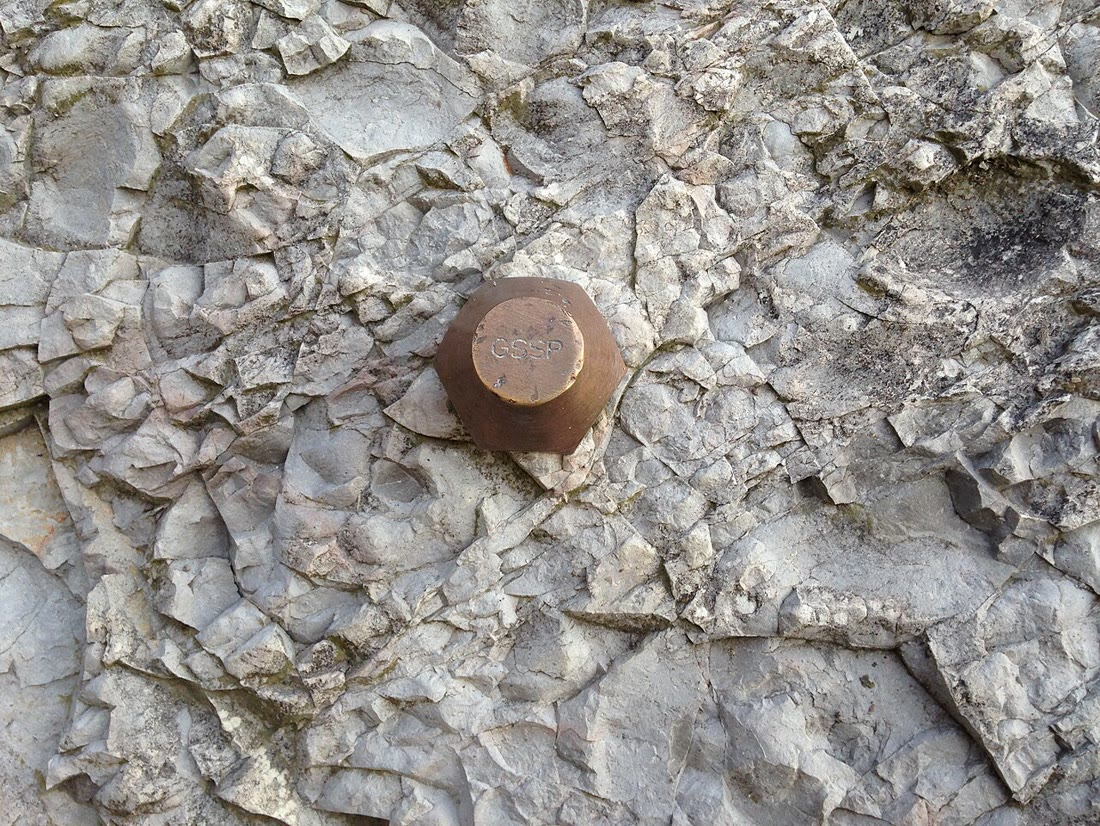
\includegraphics[width=0.62\linewidth]{images/book3/b1-golden-spike-zumaia.jpg}

{\small 祖迈亚剖面中塞兰阶的金钉：一枚刻有 GSSP 字样的青铜标志，
设于某一组最上层石灰岩层的顶部，
恰在下一组红色泥灰岩层的底部。（Josugoni，CC~BY-SA~4.0，
经维基共享资源。）}
\label{fig:b1:stratigraphic-scale:zumaia}
\end{omfigure}
% ledger: commons:zumaia-gssp, gssp:selandian

\begin{recall}
在一叠未经倒转的岩层中，每一层都比其下方的岩层年轻；
切穿岩石的构造比它所切穿的岩石年轻；
化石在各地都以相同的顺序，由老地层向新地层依次变化；
地球历史划分为代和地质时期，每个单位都有以年计的起始时间，并汇总于国际年代表中
（见第 1 册，七年级）。
\omterm{def:b1:cross-sections:log}{钻孔柱状图}记录沿深度遇到的各单位，对比则是在各柱状图之间匹配相同的单位
（见\cref{def:b1:cross-sections:log}）；\omterm{def:b1:cross-sections:unconformity}{不整合}是
侵蚀或未沉积形成的界面
（见\cref{def:b1:cross-sections:unconformity}）。\omterm{def:b1:clastic-sediments:facies}{沉积相}是一个岩石体，
其特征记录了它的\omterm{def:b1:clastic-sediments:facies}{沉积环境}
（见\cref{def:b1:clastic-sediments:facies}）。生物各册描述物种
如何出现与灭绝，以及少数几次大灭绝——在这些事件中，
其中全部物种的很大一部分在短时间内消失。
\end{recall}

\section{用三种方式划分岩层}\label{sec:b1:stratigraphic-scale:three}

地质学家记录一段悬崖时，可以用三种方式划分同一叠岩层：按岩石的物质组成、
按其所含化石，以及按岩层形成的时间。三种划分回答的问题不同，
其界线未必重合。
每一类单位的命名与定义规则
由国际协议规定。
% ledger: isg:lithostratigraphy

\begin{definition}[组、段、群]\label{def:b1:stratigraphic-scale:lithostratigraphy}
\emph{岩石地层单位}\index{岩石地层单位}是一种岩石体，
依据其岩性及其在其他岩石体中的位置加以定义和识别，
不论其时代。最基本的单位是
\emph{组}\index{组（岩石地层）}：一种岩石体，与其邻近岩石体的差别足够大，
能够在区域尺度上填图，应将整个地层柱划分为若干组。
\emph{段}\index{段 （岩石地层）}
是组内按岩性区分的命名细分单位；\emph{群}\index{群（岩石地层）}是
由两个或更多组构成的层序，
这些组具有显著的共同岩性特征。正式名称由当地地名
加上岩石级别或主导岩性构成：
凯尔砂岩、马登页岩组。
\end{definition}
% ledger: isg:lithostratigraphy

组的厚度可以不足一米，也可达数千米。
其范围仅延伸至岩性仍可辨认之处，
因此其边界随岩石走，而非随时间走。
% ledger: isg:lithostratigraphy

\begin{definition}[生物带、标准化石、首现面]\label{def:b1:stratigraphic-scale:biozone}
\emph{生物带}\index{生物带}是由其所含化石定义或表征的地层体。
\emph{延限带}\index{延限带}包含某一分类单元已知的全部产出；
\emph{间隔带}\index{间隔带}是
位于两个指定化石层位之间的地层体，例如两个分类单元的最低产出层位。
\emph{首现面}\index{首现面}（FAD）是某一分类单元的
最低产出层位，而
\emph{末现面}\index{末现面}则为其最高产出层位。
\emph{标准化石}\index{标准化石}是用于识别生物带的分类单元。
最好的标准化石分布广、数量多、易于鉴定，
且演化时限短。
\end{definition}
% ledger: isg:biostratigraphy, og:stratigraphy-principles

化石层位没有厚度；\omterm{def:b1:stratigraphic-scale:biozone}{生物带}的厚度
可为几米，也可为几百米，取决于分类单元存活期间沉积物堆积的快慢。
物种会演化，灭绝后不再重现，因此任一时代的化石组合都是唯一的。
最好的\omterm{def:b1:stratigraphic-scale:biozone}{标准化石}中有一些是微体化石，如有孔虫和牙形刺：
它们分布广、数量多，且个体小，
足以从水井的岩屑中获取。
% ledger: isg:biostratigraphy, og:stratigraphy-principles

\begin{definition}[年代地层单位与地质年代单位]\label{def:b1:stratigraphic-scale:chronostratigraphy}
\emph{年代地层单位}\index{年代地层单位}是在某一给定地质时间间隔内形成的全部岩石所构成的岩石体，
且仅包含该时间间隔内形成的岩石；
其界线为等时面。时间间隔本身称为
\emph{地质年代单位}\index{地质年代单位}。等级由小到大依次为
\emph{阶}\index{阶（年代地层）}（对应时间为期）、
\emph{统}\index{统（年代地层）}（对应时间为世）、
\emph{系}\index{系（年代地层）}（对应时间为纪）、界（对应时间为代）
和宇（对应时间为宙）；每个单位由其下一级的若干个
连续单位组成。
\end{definition}
% ledger: isg:chronostratigraphy

这两个词描述的是同一划分，一个从岩石的角度看，一个从时间的角度看
（见\cref{tab:b1:stratigraphic-scale:ranks}）：侏罗系的岩层
形成于侏罗纪，下侏罗统的岩层形成于
早侏罗世。阶是全世界公认的
最小单位。
% ledger: isg:chronostratigraphy, chart:danian

\begin{table}[htbp]
\centering
\begin{tabular}{lll}
\hline
\omterm{def:b1:stratigraphic-scale:chronostratigraphy}{年代地层单位}（岩石） & \omterm{def:b1:stratigraphic-scale:chronostratigraphy}{地质年代单位}（时间） & 实例 \\
\hline
宇 & 宙 & 显生宙 \\
界 & 代 & 新生代 \\
系 & 纪 & 古近纪 \\
统 & 世 & 古新世 \\
阶 & 期 & 丹麦阶（\qtyrange{66.00}{61.66}{\Ma}） \\
\hline
\end{tabular}
\caption{\omterm{def:b1:stratigraphic-scale:chronostratigraphy}{年代地层单位}与\omterm{def:b1:stratigraphic-scale:chronostratigraphy}{地质年代单位}的各级划分，以及
包含新生代第一个阶丹麦阶的各级单位。}
\label{tab:b1:stratigraphic-scale:ranks}
\end{table}
% ledger: isg:chronostratigraphy, chart:danian

\section{地层原理与对比}\label{sec:b1:stratigraphic-scale:principles}

在能够以年为单位给岩石定年之前，事件的先后顺序是从
岩石本身读取的。地层学的基本原理由
尼古拉斯·斯泰诺于 1669 年提出；1785 年至 1800 年间，赫顿和威廉·史密斯又
补充了以岩层作为时间间隔、以其中化石作为识别依据的做法。
% ledger: og:stratigraphy-principles, usgs:hutton-smith

\begin{definition}[地层学原理]\label{def:b1:stratigraphic-scale:principles}
\begin{enumerate}
  \item \emph{叠加原理}\index{叠加原理 }
：在未被倒转的沉积岩层序中，
        每一层都比其所覆盖的那一层年轻。
  \item \emph{原始水平律}\index{原始水平律 }
：沉积物和熔岩流
        最初是水平沉积的，或近似水平——
        在盆地边缘略有倾斜。
  \item \emph{横向连续律}\index{横向连续律 }
：在盆地内，一层岩层在各个方向上连续延伸，
        直到在盆地边缘或遇到障碍物处尖灭；
        被山谷切断的岩层在谷的另一侧继续延伸。
  \item \emph{切割律}\index{切割律 }
：凡切穿岩石的岩体或构造——
        如岩墙、断层、侵蚀面——
        均比其所切穿的岩石年轻。
  \item \emph{生物层序律}\index{生物层序律 }
：化石分类单元在各地区都以相同次序相继出现，
        因而含相同化石组合的岩层
        时代相同。
\end{enumerate}
\end{definition}
% ledger: og:stratigraphy-principles, eli:relative-dating, usgs:fossil-succession, isg:chronostratigraphy

各条原理的强弱并不相同。\omterm{def:b1:stratigraphic-scale:principles}{叠加原理}给出一种顺序，
其他方法都必须遵从。\omterm{def:b1:stratigraphic-scale:principles}{原始水平律}使倾斜的岩层
成为后期变形的记录。\omterm{def:b1:stratigraphic-scale:principles}{横向连续律}使地质学家能够
在山谷两侧画出同一岩层，并且在有限距离内，一个
沿地面追踪的层面，是现有最好的等时线。
\omterm{def:b1:stratigraphic-scale:principles}{生物层序律}是能跨越大洋的原理；下面
几段将专门讨论它。
% ledger: isg:chronostratigraphy, og:stratigraphy-principles

\subsection*{生物带对比}

依据化石的对比，是比较两个剖面中首现与末现的
次序（见下图）。两者的可靠程度并不相同。一个分类单元在某剖面中所见最高的化石
其位置取决于保存下来的数量：化石稀少时，
所发现的最后一个化石可能远低于该分类单元真正灭绝的层位，
而被侵蚀并再沉积的化石则可能出现在其上方。首现
也可能发生位移，但分布广、扩散快的分类单元
在整个盆地内大致处于同一层位。
% ledger: isg:biostratigraphy

\begin{omfigure}
\begin{tikzpicture}[font=\footnotesize, y=0.13cm]
  % section 1: 40 m, sandstone 0-14, shale 14-40
  \fill[lith sandstone] (0,0) rectangle (0.8,14);
  \fill[lith shale] (0,14) rectangle (0.8,40);
  \draw[black!70] (0,0) rectangle (0.8,40);
  \node[anchor=south, font=\small] at (1.4,41.5) {剖面 1};
  \foreach \x/\a/\b/\t in {1.1/0/27/a, 1.4/10/34/b, 1.7/20/40/c, 2.0/30/40/d} {
    \draw[line width=2.2pt, omThm] (\x,\a) -- (\x,\b);
    \node[anchor=base, font=\scriptsize] at (\x,-4.5) {\t};
  }
  \foreach \y/\z in {5/a, 15/b, 25/c, 35/d}
    \node[anchor=east, font=\scriptsize] at (-0.1,\y) {带 \z};
  \foreach \y in {10,20,30} \draw[black!50] (-1.3,\y) -- (0,\y);
  % scale bar
  \draw[thick] (-1.5,0) -- (-1.5,10) node[midway, anchor=east, font=\scriptsize] {\qty{10}{m}};
  % section 2: 24 m, sandstone 0-3, shale 3-24
  \begin{scope}[xshift=7cm]
    \fill[lith sandstone] (0,0) rectangle (0.8,3);
    \fill[lith shale] (0,3) rectangle (0.8,24);
    \draw[black!70] (0,0) rectangle (0.8,24);
    \node[anchor=south, font=\small] at (1.4,25.5) {剖面 2};
    \foreach \x/\a/\b/\t in {1.1/0/13/a, 1.4/6/20/b, 1.7/12/24/c, 2.0/18/24/d} {
      \draw[line width=2.2pt, omThm] (\x,\a) -- (\x,\b);
      \node[anchor=base, font=\scriptsize] at (\x,-4.5) {\t};
    }
    \foreach \y/\z in {3/a, 9/b, 15/c, 21/d}
      \node[anchor=west, font=\scriptsize] at (2.3,\y) {带 \z};
    \foreach \y in {6,12,18} \draw[black!50] (0.8,\y) -- (2.3,\y);
  \end{scope}
  % correlation of the first appearances
  \foreach \u/\v/\t in {10/6/b, 20/12/c, 30/18/d}
    \draw[densely dashed, omThm!70!black] (2.15,\u) -- (6.85,\v)
      node[pos=0.5, fill=white, inner sep=1pt, font=\scriptsize] {FAD \t};
\end{tikzpicture}

{\small 延限图，以及按\omterm{def:b1:stratigraphic-scale:biozone}{生物带}进行的对比（虚构的分类单元 \emph{a} 至
\emph{d}）。粗条表示各剖面中各分类单元的延限。三个
\omterm{def:b1:stratigraphic-scale:biozone}{间隔带}由 \emph{b}、\emph{c} 和 \emph{d} 的\omterm{def:b1:stratigraphic-scale:biozone}{首现面}界定，这些\omterm{def:b1:stratigraphic-scale:biozone}{首现面}
在各剖面之间相互连接（虚线）。\emph{a} 的\omterm{def:b1:stratigraphic-scale:biozone}{末现面}
在剖面~1 中落于带~\emph{c} 的上部，在剖面~2 中则靠近其底部：它是
较差的指示标志。剖面~2 中的带较薄，
那里的沉积速率较慢。}
\label{fig:b1:stratigraphic-scale:range-chart}
\end{omfigure}

\begin{method}[按生物带对比剖面]\label{met:b1:stratigraphic-scale:biozones}
\begin{enumerate}
  \item 对每个剖面，绘出各分类单元的延限随高度的变化：
        即从其最低出现层位到最高出现层位。
  \item 选取界定各带的化石层位，最好是广布分类单元的首现层位，
        且这些分类单元与\omterm{def:b1:clastic-sediments:facies}{沉积相}无关。
  \item 在每个剖面中，于这些层位处画出带的界线。
  \item 将各剖面中相同的层位逐一连接，检查这些连线
        是否相交，这符合\omterm{def:b1:stratigraphic-scale:principles}{叠加原理}的要求。
  \item 在两条连线之间，读取各带在每个剖面中的厚度；
        若某个带缺失，应先查找\omterm{def:b1:cross-sections:unconformity}{不整合}或\omterm{def:b1:clastic-sediments:facies}{沉积相}的变化，
        然后才能断定该分类单元不存在。
\end{enumerate}
\end{method}

\omterm{def:b1:stratigraphic-scale:biozone}{生物带}的可靠程度，取决于其化石与环境的无关程度。
一种只生活在砂质海岸上的双壳类，只见于砂岩中；
沿着它从一个剖面追踪到另一个剖面，追踪的是砂岩，而非时间。
因此，生物地层对比不一定是时间对比：
它可能追踪的是一个年龄随地而异的\omterm{def:b1:clastic-sediments:facies}{沉积相}。
% ledger: isg:biostratigraphy

\subsection*{穿时界线}

同一时期，不同地点沉积的物质各不相同：岸边为砂，
离岸为泥，陆架外缘缺砂处则为石灰质。
因此，一条等时线会穿过不同的岩性。
反之，沿盆地追踪的岩性界线，
未必处处都是等时线。
% ledger: og:stratigraphy-principles, isg:chronostratigraphy

\begin{definition}[穿时界线]\label{def:b1:stratigraphic-scale:diachronous}
若界线沿其\omterm{def:b1:geological-maps:attitude}{走向}的年龄随地点而变化，则称该界线为\emph{穿时的}\index{穿时的}。
组的界线与\omterm{def:b1:clastic-sediments:facies}{沉积相}的界线通常是穿时的；
而\omterm{def:b1:stratigraphic-scale:chronostratigraphy}{年代地层单位}的界线，
按定义则不是。
\end{definition}
% ledger: isg:lithostratigraphy, isg:chronostratigraphy, isg:biostratigraphy

典型的情形是海侵：\omterm{def:b1:diagenesis-basins:eustasy}{相对海平面}上升快于沉积物填满所腾出空间的速度，
于是海岸线向陆地方向移动。海滩砂在每一瞬间都沉积在海岸线上，
因此一层砂岩席随之向陆地方向扩展；
离岸的泥则覆盖其上。砂岩的顶面
便是移动海岸线的痕迹：向陆一侧较新，向海一侧较老
（见下图）。同一竖直剖面中所见的相序——砂岩位于页岩之下，页岩位于石灰岩之下——
在某一时刻重复出现于陆架上，其排列顺序与此一致；
本科三年级分册据此把它作为其\omterm{def:b1:clastic-sediments:facies}{沉积相}模型的基础。
% ledger: og:stratigraphy-principles, isg:lithostratigraphy

\begin{omfigure}
\begin{tikzpicture}[font=\footnotesize, x=1cm, y=1cm]
  % basement surface B(x) = 1.6 (1 - x/14), rising towards the land on the left
  \fill[lith granite] (0,-0.5) -- (0,1.6) -- (14,0) -- (14,-0.5) -- cycle;
  \fill[lith sandstone] (0,1.6) -- (14,0) -- (14,0.5) -- (0,2.1) -- cycle;
  \fill[lith shale] (0,2.1) -- (14,0.5) -- (14,1.5) -- (0,3.1) -- cycle;
  \fill[lith limestone] (0,3.1) -- (14,1.5) -- (14,3.6) -- (0,3.6) -- cycle;
  \draw[unconformity] (0,1.6) -- (14,0);
  \draw[black!70] (0,2.1) -- (14,0.5) (0,3.1) -- (14,1.5);
  \draw[black!70] (0,-0.5) rectangle (14,3.6);
  % time lines: horizontal, from the basement (or the left edge) to the right edge
  \foreach \y/\t in {0.6/1, 1.1/2, 1.6/3, 2.1/4, 2.6/5, 3.1/6} {
    \pgfmathsetmacro{\xs}{max(0, 14*(1-\y/1.6))}
    \draw[omThm, thick, densely dashed] (\xs,\y) -- (14,\y) node[anchor=west, text=black] {$t_\t$};
  }
  % two sections
  \foreach \x/\n in {3/1, 11/2} {
    \draw[very thick, black] (\x,-0.5) -- (\x,3.6);
    \node[anchor=south, font=\small] at (\x,3.65) {剖面 \n};
  }
  \node[fill=white, inner sep=1pt, font=\scriptsize] at (5.6,1.21) {砂岩};
  \node[fill=white, inner sep=1pt] at (12.6,1.2) {页岩};
  \node[fill=white, inner sep=1pt] at (7.0,3.25) {石灰岩};
  \node[fill=white, inner sep=1pt] at (12.0,-0.25) {基底};
  \draw[-{Stealth}, thick] (5.6,4.35) -- (3.6,4.35) node[anchor=east] {陆地};
  \draw[-{Stealth}, thick] (8.4,4.35) -- (10.4,4.35) node[anchor=west] {海};
\end{tikzpicture}

{\small 海侵期间沉积的砂岩席（示意图，竖直方向
比例已夸大）。虚线 $t_1$ 至 $t_6$ 连接等时的点，
$t_1$ 最老。当其与基底相交时，它始于其所处时间的海岸线，
向海一侧由砂过渡为泥，在较年轻的层中则过渡为石灰质。
砂岩的顶面
在剖面~2 中位于 $t_1$ 与 $t_2$ 之间，而在剖面~1 中位于 $t_3$ 与 $t_4$ 之间：
组的界线是\omterm{def:b1:stratigraphic-scale:diachronous}{穿时的}，向陆地一侧更年轻。}
\label{fig:b1:stratigraphic-scale:diachronous}
\end{omfigure}

界线的年龄沿其\omterm{def:b1:geological-maps:attitude}{走向}变化得多快？在向陆地方向缓慢抬升的滨海平原上，
答案取决于几何关系。

\begin{proposition}[海侵的速度]\label{prop:b1:stratigraphic-scale:transgression}
设滨海平原以均匀坡度 $s$ 向陆地抬升，\omterm{def:b1:diagenesis-basins:eustasy}{相对海平面}以恒定速率 $R$ 上升，
且岸边无沉积物加入。
于是海岸线向陆地方向移动，速度为
\[
  u = \frac{R}{s},
\]
跟随海岸线的界线，在向陆地方向距离为 $d$ 的一点处
比其年轻 $\Delta t = d/u = d\,s/R$。
\end{proposition}

\begin{proof}
设 $x$ 为距某一固定点的陆向距离，$z$ 为高度；
滨海平原为直线 $z = s x$，时刻 $t$ 的海面为
$z = z_0 + R t$。岸线即两者的交点：$s\,x(t) = z_0 + R t$，于是
$x(t) = (z_0 + R t)/s$，且 $\mathrm dx/\mathrm dt = R/s$。岸线到达
向陆地方向距离为 $d$ 的一点所需的时间为 $d/u = d\,s/R$。
\end{proof}

该比值很大，因为滨海平原几乎平坦。若平原坡度为 $1$ 比 $2000$，\omterm{def:b1:diagenesis-basins:eustasy}{相对海平面}
每百万年上升 \qty{10}{m}，则岸线每百万年向陆地推进 \qty{20}{km}；
悬崖上看似同一个面的砂岩顶面，
在向陆地方向 \qty{20}{km} 处便年轻一百万年。沉积物被带到岸边，
会减缓海侵，甚至使其逆转。

\subsection*{等时线}

那么，若岩性不能对比时间，化石又只能近似对比，
又由什么来对比时间呢？最好的等时线由那些在各处同时留下痕迹的事件形成。
火山灰在大范围内落下，地质上看几乎是瞬间完成的，
并同时覆盖在砂、泥与石灰岩之上：火山灰层即一条穿越相界的等时线，
常可借助\cref{ch:b1:radiometric-methods}所述的方法，
以年为单位测定其年代。地磁倒转（在本科三年级分册中讨论）
记录于多种岩石之中，一旦其顺序已知，便可在世界各地加以识别；
碳同位素的急剧变化同样如此，
例如标记伊普尔阶底界的那次变化
（见\cref{tab:b1:stratigraphic-scale:gssps}）。两个已定年的层位之间，
任一岩层的年龄可假定沉积物以
恒定速率堆积而估算得出。
% ledger: isg:chronostratigraphy

\begin{proposition}[两个已定年层位之间的年龄]\label{prop:b1:stratigraphic-scale:interpolation}
连续剖面中高度分别为 $z_1 < z_2$ 的两个层位，年龄分别为
$t_1 > t_2$。若两者之间的沉积物以恒定速率堆积，
则两者之间高度为 $z$ 的层位的年龄为
\[
  t = t_1 - f\,(t_1 - t_2), \qquad f = \frac{z - z_1}{z_2 - z_1},
\]
堆积速率为 $r = (z_2 - z_1)/(t_1 - t_2)$。若两个年龄
分别带有独立的标准不确定度 $\sigma_1$ 和 $\sigma_2$，则内插年龄
的不确定度为
\[
  \sigma_t = \sqrt{(1 - f)^2 \sigma_1^2 + f^2 \sigma_2^2}.
\]
\end{proposition}

\begin{proof}
在恒定速率 $r$ 下，高度随时间线性增长：$z - z_1 = r\,(t_1
- t)$，由于年龄向上递减。在 $z_2$ 处，$z_2 - z_1 = r\,(t_1 - t_2)$，
由此得 $r$；两式相除得 $t_1 - t = f\,(t_1 - t_2)$。年龄
是两个独立量的线性组合 $t = (1 - f)\,t_1 + f\,t_2$，
$a X + b Y$ 的方差，其中 $X$ 与 $Y$ 相互独立，为 $a^2
\operatorname{Var} X + b^2 \operatorname{Var} Y$，由此得 $\sigma_t$。
\end{proof}

不确定度在两个定年层位之间最小，且在此处从不大于
$\sigma_1$ 与 $\sigma_2$ 中的较大者。真正的限制在于假设：
沉积物是间歇性堆积的，可能在隐蔽的间断处停止，且\omterm{def:b1:diagenesis-basins:compaction}{压实}
在砂与泥中的方式不同（见\cref{prop:b1:diagenesis-basins:solid}），因此
内插年龄的精度不会超过剖面的规则性。

\section{界线层型}\label{sec:b1:stratigraphic-scale:gssp}

\omterm{def:b1:stratigraphic-scale:chronostratigraphy}{年代地层单位}先在岩石中界定，然后再定年。较早的做法是
以整个单位的一个标准剖面来描述每个阶；但一个标准剖面的顶，
与另一个在不同地点选取的标准剖面的底，可能
之间留下一段未归属的时间空档，或者彼此重叠。现代做法
仅在一个剖面的一点上界定每个单位的下界；其上界
即为下一单位的下界。因此，任何时间段都不会
落在两个单位之间，也不会同时属于两者。
% ledger: isg:stratotype, isg:chronostratigraphy

\begin{definition}[界线层型、单位层型与 GSSP]\label{def:b1:stratigraphic-scale:gssp}
称\emph{层型}\index{层型}为被指定的岩石剖面，
用作某一单位或某一界线的标准参照。\emph{单位层型}\index{单位层型}为整个单位的标准剖面；
\emph{界线层型}\index{界线层型}为包含界定两个单位之间
界线的特定点的剖面。而
\emph{全球界线层型剖面和点位}\index{全球界线层型剖面和点位（GSSP）}（GSSP）为
国际年代地层标尺中某一单位的界线层型：
在某一剖面中的单一一点，
经国际协议选定，界定某一阶的底界，
以及以该阶开始的
所有更大单位的底界。
\end{definition}
% ledger: isg:stratotype, isg:chronostratigraphy, gssp:protocol

GSSP 是岩石中的一点，而不是年龄。
其以年计的年龄即该点定年所得的最佳结果，且可在不移动该点的情况下加以修订。
剖面的选取旨在使该点便于在别处找到：界线两侧沉积连续，
绝不能选在\omterm{def:b1:cross-sections:unconformity}{不整合}处（那里缺失的时间会使界线含混），
最好为海相，富含保存良好、分布广泛的分类单元化石，
该层位处没有相变，岩层变形或蚀变轻微，便于到达并受到保护。
最重要的是，该点应置于与某一选定标志信号相吻合的层位上，
通常为某一分类单元的首现，
该层段富含其他标志信号，
如火山灰层、地磁倒转和同位素突变，借此可在远处识别该层位。
一个永久性标志，即金钉，设于该点。
% ledger: isg:chronostratigraphy, isg:stratotype, gssp:protocol

\begin{inthefield}[界线如何确定]
界线由负责该系统的分委员会所属工作组研究，该工作组比较候选剖面，
逐层记录剖面，采集其化石、火山灰层和同位素样品，
并撰写提案。提案需要一个
绝对多数——超过 \qty{60}{\%}——的分委员会有表决权成员（约二十名专家）的支持；
提案随后交由国际地层委员会的有表决权成员、执行官员
及其十七个分委员会的主席审议，
最后提交国际地质科学联合会执行委员会，
由其批准通过。研究结果随之发表，
标志物埋设于岩石之中，新确立的界线
十年内不得提议修改。
\end{inthefield}
% ledger: gssp:protocol

\begin{table}[htbp]
\centering
\small
\begin{tabular}{>{\raggedright\arraybackslash}p{2.4cm}>{\raggedright\arraybackslash}p{1.2cm}>{\raggedright\arraybackslash}p{3.7cm}>{\raggedright\arraybackslash}p{5.6cm}c}
\hline
阶底界 & 年龄（\unit{\Ma}） & 剖面 & 标志物 & 批准年份 \\
\hline
富通阶（寒武纪） & 538.8 & 加拿大纽芬兰福图角 & 遗迹化石 \emph{Trichophycus pedum} 的首现 & 1992 \\
洛赫科夫阶（泥盆纪） & 419.62 & 捷克布拉格附近的克隆克 & 笔石 \emph{Monograptus uniformis} 的首现 & 1972 \\
因杜阶（三叠纪） & 251.902 & 中国浙江煤山 & 牙形刺 \emph{Hindeodus parvus} 的首现，27c 层底部 & 2001 \\
丹麦阶（古近纪） & 66.00 & 突尼斯埃勒凯夫的瓦德杰尔法内 & 深色界线黏土层（厚 \qty{50}{cm}）底部；铱异常 & 1991 \\
西兰阶 & 61.66 & 西班牙祖迈亚 & 红色泥灰岩底部；一种超微化石类群的第二次辐射 & 2008 \\
伊普尔阶（始新世） & 56.00 & 埃及卢克索附近的达巴比亚 & 碳同位素偏移的底部 & 2003 \\
千叶阶 & 0.774 & 日本千叶 & 火山灰层底部，位于地磁倒转之下 & 2020 \\
梅加拉亚阶 & 0.0042 & 印度梅加拉亚邦马木卢洞穴 & 石笋内深 \qty{7.45}{mm} 处的一个层位 & 2018 \\
\hline
\end{tabular}
\caption{八个 GSSP。标志物为分类单元的首现、地球化学异常、
同位素偏移、地磁倒转，以及洞穴沉积中记录的
气候事件。}
\label{tab:b1:stratigraphic-scale:gssps}
\end{table}
% ledger: gssp:fortunian, gssp:lochkovian, gssp:induan, gssp:danian, gssp:selandian, gssp:ypresian, gssp:chibanian, gssp:meghalayan

\Cref{tab:b1:stratigraphic-scale:gssps} 显示所选信号的多样程度。
表中古生代和中生代的界线依据化石的首现，
即笔石和牙形刺；寒武纪底界的化石则是
遗迹化石，即动物活动留在沉积物中的痕迹，
而非动物本身。新生代的例子中，信号是化学的和
物理的：丹麦阶的铱异常、伊普尔阶的碳同位素偏移，
以及位于千叶阶标志点上方 \qty{1.1}{m} 处的地磁倒转。
表中最年轻的界线根本不在海相岩石中：梅加拉亚阶的底界
是位于石笋内的一个层位，石笋是在洞穴中生长的沉积物，记录
了距今 4200 年前的一次气候事件。
% ledger: gssp:fortunian, gssp:danian, gssp:ypresian, gssp:chibanian, gssp:meghalayan

\begin{dated}{2026}
% ledger: gssp:count, chart:stage-count
2026 年 10 月，国际地层委员会的表格列出
80 个已批准的 GSSP，另有两个待批。首个于 1972 年批准，地点在
克隆克；最近一个于 2024 年批准，当时志留纪的两条界线
此前界定于威尔士，后改定于西班牙和捷克的
新剖面。图中显生宙的 101 个阶中，21 个尚无
已批准的 GSSP，其底界仍为暂定。
\end{dated}

显生宙以下的年代表划分方式大多不同。除最年轻的
系埃迪卡拉系外，前寒武纪按协议选定的整数年龄划分，
——其划分以年数定义，而非岩石中的点位。
% ledger: isg:chronostratigraphy

\section{作为标志的大灭绝}\label{sec:b1:stratigraphic-scale:extinctions}

生物学分册把大灭绝描述为大比例物种
在地质上较短的时间内消失的时刻。对地层学而言，这类
事件是一份“礼物”：一个层位可见于每一大陆和每一海洋，
跨越此层位，化石组合彻底改变。其中两次事件界定了
显生宙的三个代。
% ledger: schulte:kpg, burgess:end-permian

\subsection*{白垩纪末}

1980 年，L.~W.~阿尔瓦雷斯、W.~阿尔瓦雷斯、F.~阿萨罗和 H.~V.~米歇尔测定了铱
——一种铂族金属，其在\omterm{def:b1:layered-earth:layers}{地壳}中的含量相对宇宙丰度而言
偏低——在跨越该界线的深海石灰岩中，
即白垩纪与第三纪之间的界线——今称
白垩纪与古近纪之间的界线，即 K--Pg 界线。他们发现铱在意大利
比本底富集约 30 倍，在丹麦为 160 倍，在新西兰为 20 倍，
恰好位于灭绝层位。他们提出，一颗\omterm{def:b1:comparative-planetology:small-bodies}{小行星}
直径约 $\qty{10}{km}$，上下浮动约 4 千米，撞击了地球，
并将相当于自身质量 60 倍的碎岩抛入大气层；尘埃
会扩散至全球，遮暗天空。他们还指出，界线处的黏土
化学成分不同于上下石灰岩中的黏土。
% ledger: alvarez:iridium

后续研究将该界线与单一撞击事件相联系，即希克苏鲁伯撞击。氩–氩测年
将该撞击与界线及其灭绝的时间定在 \num{32000}
年之内，一篇证据综述认为该撞击引发了
灭绝，而这次灭绝也恰逢印度大规模玄武岩喷发的
时期。丹麦阶底界 GSSP——即古近纪及
整个新生代的底界——定于突尼斯埃勒凯夫深色界线黏土的底部，
即铱异常层位。同一界线也可在陆地上见到，
位于科罗拉多州（见下图）。
% ledger: renne:kpg, schulte:kpg, gssp:danian, commons:kt-tlsp

\begin{omfigure}
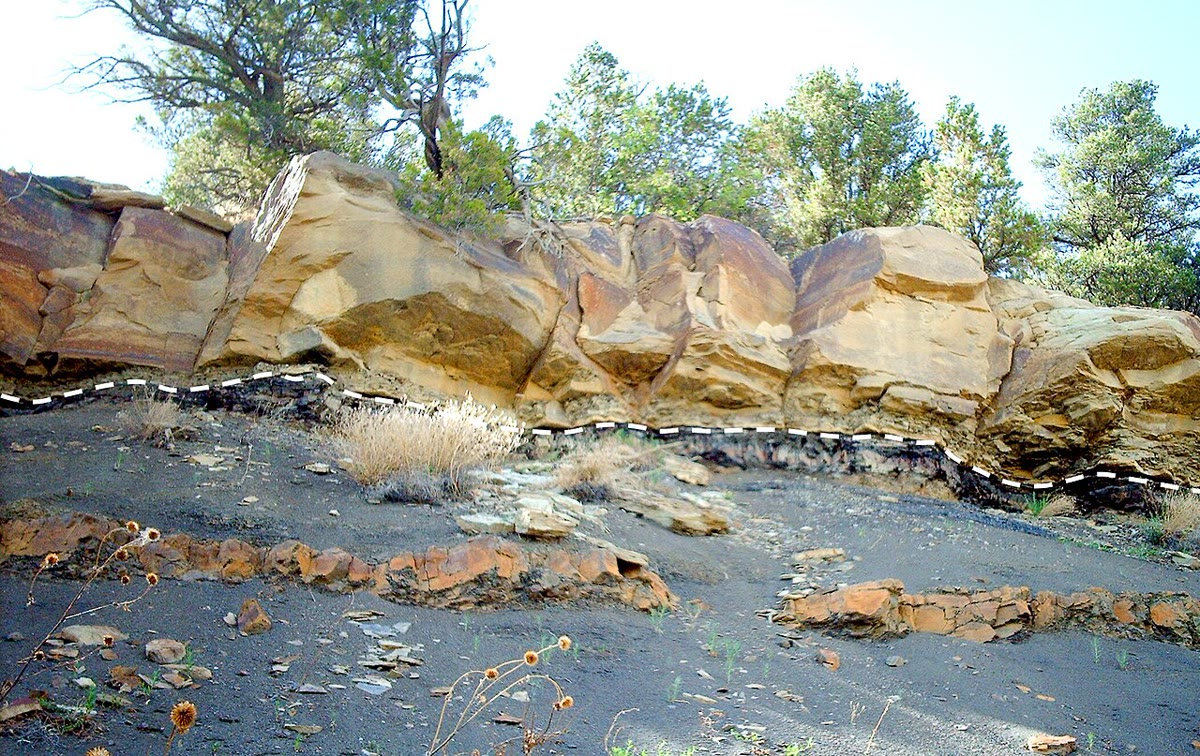
\includegraphics[width=0.78\linewidth]{images/book3/b1-kpg-boundary-trinidad.jpg}

{\small 白垩纪与古近纪之间的界线，以
虚线标示，位于科罗拉多州特立尼达湖州立公园：上部为砂岩，
下部及沿界线为深色岩层。（Nationalparks, CC~BY-SA~2.5,
经维基共享资源；虚线见于原图。）}
\label{fig:b1:stratigraphic-scale:kpg}
\end{omfigure}
% ledger: commons:kt-tlsp

\subsection*{二叠纪末}

二叠纪末的灭绝，是过去五亿年间海洋与陆地生命
损失最严重的一次。在中国煤山，即
三叠纪底界 GSSP 所在的剖面，五层火山灰层已
以锆石铀–铅法测定，它们将灭绝界定在
\qty[uncertainty-mode=separate]{251.941(37)}{\Ma} 与 \qty[uncertainty-mode=separate]{251.880(31)}{\Ma} 之间，时间间隔为
\num[uncertainty-mode=separate]{60 \pm 48} 千年。灭绝之前，碳酸盐的
碳同位素出现急剧负向偏移 \qty{3}{\permil}，此后碳循环
在约 \num{500} 千年间保持不稳定。
% ledger: burgess:end-permian, gssp:induan

三叠纪底界本身，\qty[uncertainty-mode=separate]{251.902(24)}{\Ma}，并非
定在灭绝处，而是定在牙形刺 \emph{Hindeodus parvus} 的首现，
该层位落在煤山测年所限定的灭绝区间之内。
灭绝事件即一组末现，保存作用会使其模糊；一个知名物种的首现
则能划出更清晰的界线。两次灭绝的成因——
一次撞击、大规模玄武岩省——是本科二年级分册的主题。
% ledger: gssp:induan, isg:biostratigraphy, burgess:end-permian

\section{国际年代地层表}\label{sec:b1:stratigraphic-scale:chart}

国际年代地层表汇集了从宇到阶的全部单位，
于一表中列出各单位的名称、底界年龄（以百万年计）及其不确定度、
由经批准的 GSSP 定义的各底界标记，
以及各单位的标准颜色（采用世界\omterm{def:b1:geological-maps:geological-map}{地质图}委员会的颜色标准）。
显生宙部分
仅保留其代与纪，
依据年代表本身的数值绘于下方。
% ledger: ics:base.Paleozoic, ics:colour.Paleozoic, gssp:count

\begin{omfigure}
\begin{tikzpicture}[font=\footnotesize]
\begin{axis}[y dir=reverse, ymin=0, ymax=538.8, xmin=0, xmax=6.2,
  width=6.6cm, height=11cm, scale only axis, clip=false,
  axis x line=none, axis y line*=left, ytick={0,100,...,500},
  ylabel={年龄 (\unit{\Ma})}, tick label style={font=\scriptsize}]
  \pgfplotsinvokeforeach{Paleozoic,Mesozoic,Cenozoic,Cambrian,Ordovician,Silurian,Devonian,Carboniferous,Permian,Triassic,Jurassic,Cretaceous,Paleogene,Neogene,Quaternary}{
    \addplot[fill=ics#1, draw=black!70, line width=0.3pt] table[x=x, y=age] {figdata/out/bachelor-1-ics_chart-bar-#1.dat};}
  \addplot[draw=none, point meta=explicit symbolic, opacity=0, forget plot]
    table[x=x, y=age, meta=name] {figdata/out/bachelor-1-ics_chart-eras.dat};
  \node[anchor=center, rotate=90, font=\scriptsize\bfseries] at (axis cs:0.5,395.351) {古生代};
  \node[anchor=center, rotate=90, font=\scriptsize\bfseries] at (axis cs:0.5,158.951) {中生代};
  \node[anchor=center, rotate=90, font=\scriptsize\bfseries] at (axis cs:0.5,33) {新生代};
  \addplot[draw=none, point meta=explicit symbolic, opacity=0, forget plot]
    table[x=x, y=age, meta=name] {figdata/out/bachelor-1-ics_chart-periods.dat};
  \node[anchor=center, font=\scriptsize] at (axis cs:2,512.825) {寒武纪};
  \node[anchor=center, font=\scriptsize] at (axis cs:2,464.975) {奥陶纪};
  \node[anchor=center, font=\scriptsize] at (axis cs:2,431.36) {志留纪};
  \node[anchor=center, font=\scriptsize] at (axis cs:2,389.24) {泥盆纪};
  \node[anchor=center, font=\scriptsize] at (axis cs:2,328.88) {石炭纪};
  \node[anchor=center, font=\scriptsize] at (axis cs:2,275.401) {二叠纪};
  \node[anchor=center, font=\scriptsize] at (axis cs:2,226.651) {三叠纪};
  \node[anchor=center, font=\scriptsize] at (axis cs:2,172.25) {侏罗纪};
  \node[anchor=center, font=\scriptsize] at (axis cs:2,104.55) {白垩纪};
  \node[anchor=center, font=\scriptsize] at (axis cs:2,44.52) {古近纪};
  \node[anchor=center, font=\scriptsize] at (axis cs:2,12.81) {新近纪};
  \addplot[mark=-, mark size=3pt, only marks, nodes near coords, point meta=explicit symbolic,
    every node near coord/.style={anchor=west, xshift=1pt, font=\scriptsize}]
    table[x=x, y=age, meta=lab] {figdata/out/bachelor-1-ics_chart-bases.dat};
  \addplot[only marks, mark=triangle*, mark size=3pt, mark options={rotate=90, fill=omThm, draw=omThm}, point meta=explicit symbolic]
    table[x expr=\thisrow{x}+1.75, y=age, meta=name] {figdata/out/bachelor-1-ics_chart-events.dat};
  \node[anchor=west, xshift=3pt, font=\scriptsize, text=omThm] at (axis cs:4.75,251.902) {二叠纪末};
  \node[anchor=west, xshift=3pt, font=\scriptsize, text=omThm] at (axis cs:4.75,66) {白垩纪末};
  \node[anchor=south, font=\scriptsize] at (axis cs:2,0) {第四纪};
  \node[anchor=west, font=\scriptsize] at (axis cs:3.0,-14) {0};
  \node[anchor=south, font=\scriptsize\itshape] at (axis cs:0.5,-30) {代};
  \node[anchor=south, font=\scriptsize\itshape] at (axis cs:2,-30) {纪};
  \node[anchor=south, font=\scriptsize\itshape] at (axis cs:3.5,-30) {底界 (\unit{\Ma})};
\end{axis}
\end{tikzpicture}

{\small 国际年代地层表上的显生宙，其三个代与十二个纪，按比例绘出，
采用表中颜色，并标出各纪底界的年龄（略去不确定度）。
三角形标出两个大灭绝层位的底界。第四纪长
\qty{2.58}{\Ma}，
为顶部的细带。}
\label{fig:b1:stratigraphic-scale:chart}
\end{omfigure}
% computed in figdata/bachelor-1/ics_chart.py; ledger: ics:base.Cambrian, ics:colour.Cambrian (every ics base and colour row of the eras and periods), burgess:end-permian, alvarez:iridium

各纪的长短相差悬殊（见上图）。白垩纪持续了
\qty{77.1}{\Ma}，新近纪为 \qty{20.46}{\Ma}，第四纪仅为
\qty{2.58}{\Ma}；十二个纪的平均值为 \qty{44.9}{\Ma}。
这种不均衡是历史遗留的：各系的名称是在早期分类中确定的，
那时尚无岩石能以年为单位测定年龄。有的名称表示位置（古近纪、新近纪、第四纪）——
有的表示岩石（石炭纪、白垩纪），有的取自民族或地名（奥陶纪、志留纪、泥盆纪、二叠纪）——
而年代表保留了这些名称，同时以 GSSP 定义各底界。
以年计的年龄来自界线附近火山岩的同位素测年，
例如煤山的火山灰层（\cref{ch:b1:radiometric-methods}），
并按\cref{prop:b1:stratigraphic-scale:interpolation}所述方法内插；
年代表的新版本可能会修改某一年龄，
而 GSSP 的位置保持不变。
% ledger: ics:base.Cretaceous, ics:base.Neogene, ics:base.Quaternary, isg:chronostratigraphy, burgess:end-permian

\begin{dated}{2024}
% ledger: iugs:anthropocene
人类世是 2001 年提出的名称，用于指代
一个以人类活动为标志的新时间间隔，自 2009 年起
由第四纪地层学分会下属的一个工作组进行研究。
2023 年底，该工作组提议设立一个统，始于约 1950 年，
其 GSSP 位于安大略省克劳福德湖的沉积物中。
分会投票于 2024 年 3 月 4 日结束，否决了该提议：赞成 4 票，反对 12 票，
弃权 3 票，另有 3 名成员未投票。国际地层委员会的有表决权成员
承认了该投票结果。人类世并非年代表中的一个单位；它仍是一个非正式术语，但使用广泛。
\end{dated}

\section{练习}

\begin{exercise}[$\star$]\label{exo:b1:stratigraphic-scale:1}
判断下列每个名称属于\omterm{def:b1:stratigraphic-scale:lithostratigraphy}{岩石地层单位}、生物地层单位、\omterm{def:b1:stratigraphic-scale:chronostratigraphy}{年代地层单位}
还是\omterm{def:b1:stratigraphic-scale:chronostratigraphy}{地质年代单位}，并在其有级别时给出该级别：(a)~侏罗系；
(b)~马登页岩组；(c)~早白垩世；(d)~\emph{Hindeodus parvus} 带；
(e)~丹麦阶；(f)~古新世；
(g)~马登页岩中的一个砂岩段。
% ledger: isg:lithostratigraphy, isg:biostratigraphy, isg:chronostratigraphy
\end{exercise}

\begin{exercise}[$\star$]\label{exo:b1:stratigraphic-scale:2}
利用年代表图中各代的底界（寒武纪、三叠纪和古近纪的底界），
计算古生代、中生代和新生代的时长，
以及各代占显生宙的份额。
显生宙整体占自冥古宙底界
（\qty{4567}{\Ma}）以来时间的多大份额？
% ledger: ics:base.Paleozoic, ics:base.Mesozoic, ics:base.Cenozoic, ics:base.Hadean
\end{exercise}

\begin{exercise}[$\star$]\label{exo:b1:stratigraphic-scale:3}
一个悬崖自下而上显示：岩层 A、B、C 和 D，\omterm{def:b1:geological-maps:attitude}{倾角}为 \ang{40}；岩墙
E 切穿 A 至 D；侵蚀面切穿 D 的顶部和岩墙；其上为水平岩层 F 和 G；
一条断层错断了 A 至 F，但未错断 G。将这些事件按先后排列，
并说明每一步所依据的原理。
\end{exercise}

\begin{exercise}[$\star$]\label{exo:b1:stratigraphic-scale:4}
页岩中相距 \qty{30}{m} 的两层火山灰层，年龄分别为 \qty{85.40}{\Ma}（下层）
和 \qty{84.60}{\Ma}（上层）。某\omterm{def:b1:stratigraphic-scale:biozone}{标准化石}的首现位于下层火山灰之上 \qty{12}{m} 处。
求沉积速率和该首现的年龄，
并假设速率常数为定值。
\end{exercise}

\begin{exercise}[$\star\star$]\label{exo:b1:stratigraphic-scale:5}
某剖面中有四个分类单元，其延限（高度单位为米）为：A 0--34，
B 12--50，C 26--62，D 41--70。(a)~绘制延限图。
(b)~给出 B 与 C 的共同\omterm{def:b1:stratigraphic-scale:biozone}{延限带}的范围及厚度，以及 B 与 D
首现之间的\omterm{def:b1:stratigraphic-scale:biozone}{间隔带}的范围及厚度。(c)~在第二个剖面中，B 位于
3 至 15~m，C 位于 9 至 22~m，此外别无所知。(b)中的哪些带界
可以在该处识别，哪些不能？哪些层位可以在两个剖面之间
最有把握地对比？
\end{exercise}

\begin{exercise}[$\star\star$]\label{exo:b1:stratigraphic-scale:6}
海侵期间，海岸线以 \qty{20}{km} 每百万年
的速度向陆地移动。(a)~海岸砂岩顶面的年龄在沿海侵方向
相距 \qty{60}{km} 的两口井之间相差多少？
(b)~海岸线经过靠海一侧的井之后一百万年，落下一层火山灰。该处的近海泥以
\qty{30}{m} 每百万年的速率堆积，此处火山灰层位于砂岩顶面以上多远？
(c)~火山灰落下时，海岸线位于何处？
在陆侧井中，火山灰位于砂岩之上还是之下？
为何在那里可能根本找不到它？
请用示意图加以说明。
\end{exercise}

\begin{exercise}[$\star\star$]\label{exo:b1:stratigraphic-scale:7}
(a)~计算洛赫科夫阶与印度阶底界的年龄及其
相对不确定度（以百分数表示）。其中洛赫科夫阶为 \qty[uncertainty-mode=separate]{419.62(136)}{\Ma}，印度阶为 \qty[uncertainty-mode=separate]{251.902(24)}{\Ma}。
并试说明二者差异如此之大的原因。(b)~由煤山剖面夹住二叠纪末大灭绝的两个年龄，
\qty[uncertainty-mode=separate]{251.941(37)}{\Ma} 与
\qty[uncertainty-mode=separate]{251.880(31)}{\Ma}，重新计算灭绝持续时间及其
不确定度，假定两个误差相互独立；并与已发表的
\num[uncertainty-mode=separate]{60 \pm 48} 千年相比较。
% ledger: ics:base.Devonian, gssp:induan, burgess:end-permian
\end{exercise}

\begin{exercise}[$\star\star$]\label{exo:b1:stratigraphic-scale:8}
将 1980 年假想的\omterm{def:b1:comparative-planetology:small-bodies}{小行星}视为直径为 \qty{10}{km} 的球体，密度为
\qty{3000}{kg.m^{-3}}（假定值），抛射出的尘埃质量为\omterm{def:b1:comparative-planetology:small-bodies}{小行星}质量的 60 倍。
(a)~计算\omterm{def:b1:comparative-planetology:small-bodies}{小行星}与尘埃的质量。(b)~将尘埃均匀铺展于整个地球表面，
（地球直径 \qty{12756}{km}），每平方米上落下的质量为多少？
(c)~若以 \qty{2500}{kg.m^{-3}} 的密度沉积，该层厚度为多少？
(d)~对直径分别为 \qty{6}{km} 与 \qty{14}{km} 的情形重复(c)，以给出估计的范围；
并与丹麦阶\omterm{def:b1:stratigraphic-scale:gssp}{全球界线层型剖面和点位}处界线黏土的厚度相比较。
% ledger: alvarez:iridium, planet:Earth.diameter, gssp:danian
\end{exercise}

\begin{exercise}[$\star\star$]\label{exo:b1:stratigraphic-scale:9}
(a)~某压缩层序中沉积速率为 \qty{2}{m} 每百万年，
对应二叠纪末大灭绝、历时 \num{60} 千年的区间，其厚度为多少？
若分别取其不确定度所允许的最短与最长历时，
厚度各为多少？(b)~某深海剖面沉积速率为
\qty{10}{m} 每百万年，长 \num{32000} 年的区间厚度为多少，
该区间内撞击与 K--Pg 界线同时发生。(c)~这些数字说明了什么？
对研究灭绝事件时的剖面取样有何启示？
% ledger: burgess:end-permian, renne:kpg
\end{exercise}

\begin{exercise}[$\star\star\star$]\label{exo:b1:stratigraphic-scale:10}
某滨海平原坡降为 $1$ 比 $2000$，\omterm{def:b1:diagenesis-basins:eustasy}{相对海平面}以
\qty{10}{m} 每百万年的速率上升。(a)~利用
\cref{prop:b1:stratigraphic-scale:transgression}，海岸线向陆地移动的速率为多少，
而海岸砂岩顶面的年龄
在相距 \qty{30}{km} 的两口井之间相差多少？(b)~现有沉积物被输送至海岸，
使海岸处的滨海平原以每百万年 $a$ 米的速率向上加积。
试证明海岸线以 $(R - a)/s$ 的速率向陆地移动，只要 $a < R$。
$a > R$ 时会怎样？(c)~试解释为何一个年龄变化达一百万年的砂岩顶面，
在单一悬崖中看上去
恰与一个等时面相同。
\end{exercise}

\begin{exercise}[$\star\star\star$]\label{exo:b1:stratigraphic-scale:11}
某剖面中两层火山灰分别位于 \qty{10}{m} 与 \qty{50}{m} 处，测年分别为
\qty[uncertainty-mode=separate]{100.50(5)}{\Ma} 与 \qty[uncertainty-mode=separate]{99.70(3)}{\Ma}。(a)~求
\qty{25}{m} 处层位的年龄及其不确定度，
利用\cref{prop:b1:stratigraphic-scale:interpolation}插值求得。(b)~两层火山灰之间，
何处不确定度最小？求 $f$ 取何值时 $\sigma_t$ 最小，
以及该最小值。(c)~证明在两层之间 $\sigma_t$ 不超过 $\sigma_1$ 与
$\sigma_2$ 中的较大者。
\end{exercise}

\begin{exercise}[$\star\star\star$]\label{exo:b1:stratigraphic-scale:12}
一口井穿过一层均质页岩。测年为 \qty{30.0}{\Ma} 的火山灰位于
\qty{1000}{m} 深处，另一层测年为 \qty{29.0}{\Ma} 的火山灰位于 \qty{200}{m} 处，阶界
位于 \qty{600}{m} 处。(a)~由深度插值求阶界的年龄。(b)~
假定颗粒（而非孔隙）以恒定速率沉积。利用
\cref{tab:b1:diagenesis-basins:athy} 中的页岩数据以及
\cref{prop:b1:diagenesis-basins:solid}，计算每层火山灰与阶界之间的固体厚度，
并按此厚度比例重新插值求年龄。
(c)~两种估计相差多少千年，
哪一种较好？
% ledger: pybacktrack:compaction
\end{exercise}

\section{问题：跨盆地对比三个剖面}

\begin{problem}[{周末问题——化石、火山灰层与穿时的
砂岩如何共同确定一个阶界的年代}]
\label{pb:b1:stratigraphic-scale:1}
% values: calc/ch24.py; the basin, its sections, its taxa (Vardenoceras and Ostreola) and its ash ages are invented
沿一条穿过虚构盆地的线测量了三个剖面：西侧为 A，
B 位于 A 以东 \qty{25}{km}，C 位于 B 以东 \qty{20}{km}。每个剖面中，凯尔砂岩
之上覆盖着马登页岩。表中高度为各剖面底部
以上的高度（单位为米）：
\begin{center}
\small
\begin{tabular}{lccc}
\hline
 & A & B & C \\
\hline
实测总厚度                       & 80.0 & 66.0 & 32.0 \\
凯尔砂岩顶面                    & 45.0 & 20.0 & 6.0 \\
火山灰层 1（测年 \qty[uncertainty-mode=separate]{152.40(4)}{\Ma}）       & 5.0  & 8.0  & 3.0 \\
火山灰层 2（测年 \qty[uncertainty-mode=separate]{151.20(4)}{\Ma}）       & 71.0 & 56.0 & 27.0 \\
\emph{Vardenoceras medium} 首现 & 36.6 & 31.2 & 14.8 \\
\emph{Vardenoceras ultimum} 首现 & 65.8 & 52.0 & 24.8 \\
\emph{Vardenoceras primum} 末现   & 49.0 & 40.0 & 19.0 \\
\hline
\end{tabular}
\end{center}
\emph{V.~primum} 自每个剖面底部起即有发现。双壳类
\emph{Ostreola} 仅见于三个剖面的凯尔砂岩中。定义了三个\omterm{def:b1:stratigraphic-scale:biozone}{间隔带}，
分别为：带~1 止于
\emph{V.~medium} 的首现，带~2 止于 \emph{V.~ultimum} 的首现，带~3 位于其上。阶界
在别处的\omterm{def:b1:stratigraphic-scale:gssp}{全球界线层型剖面和点位}上，
以 \emph{V.~medium} 的首现定义。

\medskip
\noindent\textbf{第一部分——\omterm{def:b1:stratigraphic-scale:biozone}{生物带}。}
\begin{enumerate}
  \item 在同一竖直比例尺下，将三个剖面并排画出，
        标出凯尔砂岩、火山灰层和各带界线。
  \item 给出每个剖面中带~2 的厚度，以及
        带~3 中已记录部分的厚度。
  \item 为什么三个剖面中都无法确定带~1 的底界？
  \item 为什么 \emph{Ostreola} 虽然十分常见，却是一种较差的\omterm{def:b1:stratigraphic-scale:biozone}{标准化石}？
  \item \emph{V.~primum} 的末现在每个剖面中位于哪一个带内，
        它能否作为第四条带界线？
  \item 以 \emph{V.~medium} 与
        \emph{V.~ultimum} 的首现为依据对剖面进行对比。带~2 的厚度之比
        说明了什么？
\end{enumerate}

\noindent\textbf{第二部分——凯尔砂岩。}
\begin{enumerate}[resume]
  \item 在每个剖面中，凯尔砂岩的顶部位于哪个带内？
  \item 凯尔砂岩的顶面是否为等时面？海岸线曾向哪个方向
        移动？这是哪一类事件？
  \item 三个剖面中，火山灰层~1 均位于凯尔砂岩中，火山灰层~2 位于
        马登页岩中。为什么火山灰层比
        组界更适合作为时间线？
  \item 在
        \cref{def:b1:stratigraphic-scale:principles}中的哪些原理可以支持沿
        单一火山灰层从 A 追踪到 C？
\end{enumerate}

\noindent\textbf{第三部分——速率。}
\begin{enumerate}[resume]
  \item 计算每个剖面中两层火山灰层之间的
        堆积速率，单位为米每百万年。
  \item 试说明速率为何从 A 到 C 逐渐降低。
  \item 一个厚 \qty{10}{cm} 的样品在每个剖面中代表
        多少年？哪个剖面的时间分辨率最高？
  \item 假定速率恒定，计算每个剖面中凯尔砂岩
        顶部的年龄。
  \item 计算海岸线在 C 与 B 之间以及 B 与 A 之间的
        移动速度，单位为千米每百万年。海侵速度是加快
        还是减慢了？
  \item 计算每个剖面中 \emph{V.~ultimum} 首现的
        年龄。
  \item 第~16 题中的三个年龄，在火山灰
        定年数据的不确定度范围内是否一致？这对首现说明了什么？
\end{enumerate}

\noindent\textbf{第四部分——界线的年龄。}
\begin{enumerate}[resume]
  \item 在每个剖面中内插求出
        \emph{V.~medium} 首现的年龄。
  \item 由火山灰定年数据的不确定度，利用
        \cref{prop:b1:stratigraphic-scale:interpolation}计算每个年龄的不确定度。
  \item 计算三个年龄的平均值及其离散程度。
        离散程度比第~19 题的不确定度更大还是更小？
  \item 在剖面~A 中，\emph{V.~medium} 的首现位于凯尔
        砂岩中，在 B 和 C 中则位于马登页岩中。火山灰层之间
        岩性的变化如何会使 A 中的内插产生偏差？
  \item 三个剖面中哪一个最适合作为\omterm{def:b1:stratigraphic-scale:gssp}{界线层型}，
        为什么？哪一个最不适合？
  \item 带~2 持续了多长时间？
  \item 界线的内插年龄是多少？
\end{enumerate}
\end{problem}
